\section{Mechanism of Forking}
\label{sec:mechanism}

Section~\ref{sec:empirical} left two questions: why the gap follows a power law in context frequency, and why replay keeps widening it. We answer the first with continuation \emph{coverage} and the second with \emph{crowding-out} inside context subspaces, then show that the $n$-gram module is what makes those subspaces independent.

\subsection{Coverage: novel continuations and the frequency law}
\label{sec:coverage}
Section~\ref{sec:forking-factors} found that low-frequency contexts carry most of the gap. Overfitting, in general, hurts on the validation samples that training never showed; in next-token prediction these are the positions whose context occurs in training but whose true continuation never followed it there---\emph{seen context, novel continuation}. Such positions make up 31\% of the validation stream when contexts are counted as bigrams, yet they carry 73\% of the both-table model's excess validation loss over the no-gram control at step 1000; adding the seen continuations of rare contexts ($F\le 31$) brings this to 77\%, and at trigram granularity novel continuations account for essentially all of it (Appendix~\ref{app:novel-share}). Replay reinforces the continuations a context was seen with but supplies no evidence about the others, so we attribute the gap at a context to its novel-continuation mass times a per-epoch damage factor $g_j$; averaged over contexts with the same training count $F$,
\begin{equation}
\gap_j(F)\approx g_j\,M(F).
\label{eq:gap_j}
\end{equation}
The measured gaps of Figure~\ref{fig:frequency} fit
\begin{equation}
\gap^{\mathrm{bi}}(F)\approx 7.21\,F^{-0.233},\qquad
\gap^{\mathrm{tri}}(F)\approx 3.76\,F^{-0.318}.
\label{eq:gap-fits}
\end{equation}
Natural language supplies the power law. Good--Turing estimation \citep{good1953population,gale1995good} gives the probability that a context seen $F$ times is followed by an unseen continuation as $\widehat M(F)=N_1(F)/F$, where $N_1$ counts continuation types that followed it exactly once---a statistic of the text, not of any model. If conditional continuation frequencies have a Zipf-like tail $p_{(r)}\propto r^{-s}$, this missing mass decays as $F^{-\alpha}$ with $\alpha=1-1/s$ \citep{gnedin2007occupancy}; the derivation is in Appendix~\ref{app:math}. On our corpus the estimate, averaged over the contexts at each count $F$, is a clean power law over the window $F\le10^3$ in which the gap is measured (Appendix Figure~\ref{fig:b_t_MF}),
\begin{equation}
\widehat M^{\mathrm{bi}}(F)\approx 0.95\,F^{-0.287},\qquad
\widehat M^{\mathrm{tri}}(F)\approx 0.97\,F^{-0.314}.
\label{eq:gt-fits}
\end{equation}
The exponents read off corpus counts thus land within $0.05$ (bigram) and $0.01$ (trigram) of those the model produces, and a single damage factor $g$ per branch turns $\widehat M(F)$ into the measured gap: across the seven observed frequency bins the ratio $\operatorname{gap}/\widehat M$ is constant to within 9\% and 18\% (Appendix Figure~\ref{fig:gt-kernel}). The frequency law of Section~\ref{sec:forking-factors} is therefore a property of the corpus: rare contexts have more of their continuation mass unseen. Coverage does not account for everything---about a quarter of the excess loss falls on seen continuations of frequent contexts, and for trigram contexts $g$ drifts slightly with $F$ (Appendix~\ref{app:gt-fits})---but it fixes the exponent.

\begin{figure}[!t]
\centering
\begin{subfigure}[b]{0.58\linewidth}
\centering
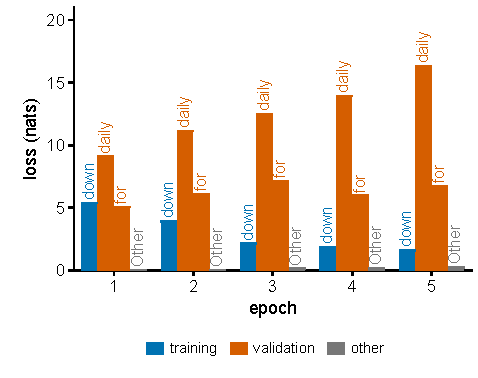
\includegraphics[width=\linewidth]{walk_their_dog_loss.pdf}
\subcaption{}
\label{fig:walk-their-dog}
\end{subfigure}\hfill
\begin{subfigure}[b]{0.38\linewidth}
\centering
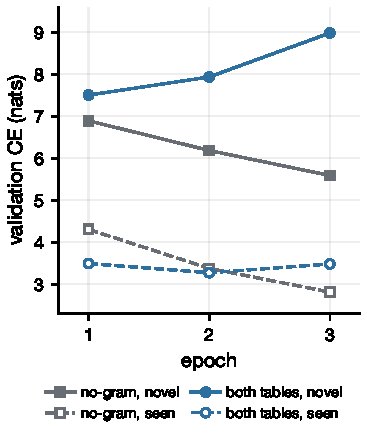
\includegraphics[width=\linewidth]{fig09_crowd_ce_seen_novel.pdf}
\subcaption{}
\label{fig:crowd-ce}
\end{subfigure}
\caption{Crowding-out: (a) context-only continuation losses for ``walk their dog''; (b) validation cross-entropy of train-seen and novel continuations, pooled over contexts.}
\label{fig:crowding}
\end{figure}

\subsection{Crowding-out: replay sharpens each context subspace}
\label{sec:sharpening}
Coverage says what is missing. The more important questions are why replay turns the missing coverage into loss, why the $n$-gram module is needed for it, and how the damage evolves with the number of passes. Our answer is that forking is ordinary overfitting confined to very small problems. For a context $c_i$, call the next-token logits computed from it its \emph{context subspace}, and split the vocabulary into the continuations of $c_i$ seen in training, those that appear only in validation, and the rest (Appendix~\ref{app:crowding-derivation}). If training shows a single continuation $C$, the loss in that subspace is $-\ln p_C$; a gradient step raises the logit of $C$ by $\eta(1-p_C)$ and, through the softmax, lowers every other logit by $\eta p_v$. Mass flows from the unseen continuations onto the seen one, so the validation loss on plausible-but-unseen continuations rises by the same shift that lowers the training loss, and the seen-to-unseen odds grow by a factor above one at every pass with nothing to stop them while $p_C<1$ (Appendix Equation~\eqref{eq:zt}). We call this \emph{crowding-out}; it is the growth of the damage factor $g_j$ with replay.

Figure~\ref{fig:walk-their-dog} shows the picture on one context. ``walk their dog'' is followed by \emph{down} once in training and, in the fixed validation window, once each by \emph{daily} and \emph{for}. Probed with context-only input, the probability of \emph{down} rises by more than an order of magnitude over five passes while \emph{daily} and \emph{for} are compressed---\emph{daily} by orders of magnitude---and so is the total mass outside the continuations observed in either sample. Figure~\ref{fig:crowd-ce} shows that the context is typical. Pooling validation positions whose bigram context occurs in training, split by whether the continuation was seen there (405{,}058 positions) or not (158{,}790), both models do well on seen continuations: the control's cross-entropy falls from 4.3 to 2.8 nats and the both-table model's stays near 3.4. On novel continuations they diverge: the control still improves, 6.9 to 5.6 nats, while the both-table model deteriorates from 7.5 to 9.0 with a step at every epoch boundary---the staircase of Figure~\ref{fig:staircase}. Crowding-out also explains why freezing the tables does not stop forking (Section~\ref{sec:interventions}): the subspace coordinate is already in place, and the backbone can continue the descent on its own.

In sum, coverage sets the size of the target ($F^{-\alpha}$, fixed by the corpus) and crowding-out sets the damage per pass ($g_j$, growing with replay). Their product is the gap.

\subsection{The n-gram module partitions the model into context subspaces}
\label{sec:context-locality}
Section~\ref{sec:sharpening} treats each context subspace as evolving on its own. That independence is what the $n$-gram module provides. A next token depends heavily on the few tokens before it, and over-encoding makes this dependence explicit: the table gives each context a private coordinate that the backbone can read out without disturbing other contexts. One symptom is that the model becomes far more confident than it is accurate. At epoch 3 the both-table model's predictive entropy on validation is 2.93 nats against a cross-entropy of 5.26, whereas the no-gram control's are 3.59 and 3.58 (same runs as Figure~\ref{fig:crowd-ce}); low-entropy predictions paired with high cross-entropy are the signature of a sharpened model that has committed to few continuations per context \citep{carlsson2025hyperfitting}.

\begin{figure}[!htbp]
\centering
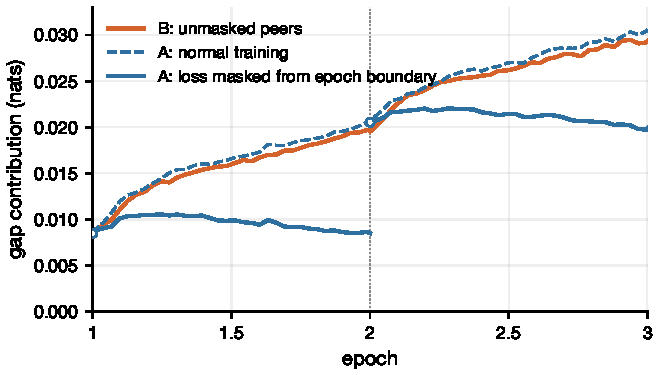
\includegraphics[width=0.62\linewidth]{fig07_context_mask.pdf}
\caption{Random context loss masking: gap contribution of 2\% of training trigram contexts ($A$) whose loss is excluded from an epoch boundary onward, against unmasked peers ($B$) and normal training.}
\label{fig:context-subspace-mask}
\end{figure}

We test the independence directly. We randomly select 2\% of training trigram contexts, $A$, and exclude their next-token loss from epoch~1 or epoch~2 onward, keeping inputs, trainable parameters, and the loss denominator unchanged; $B$ is a disjoint random unmasked peer set, and each run is paired with normal training from the same checkpoint. Figure~\ref{fig:context-subspace-mask} plots the gap contribution $C_S(t)=\sum_{i\in S}q_i[\bar\ell_{\mathrm{val},i}(t)-\bar\ell_{\mathrm{tr},i}(t)]$, with $q_i$ the context's fixed share of validation positions. As soon as their loss is masked, the contexts in $A$ stop accumulating gap and stay flat for the rest of the epoch, while $B$ keeps climbing on top of normal training. Updates driven by other contexts therefore do not move a context's own gap: the gap is generated inside each subspace by its own replay, which is exactly the dynamics assumed in Section~\ref{sec:sharpening}.
\pending{Planned companion panel: KL divergence of the masked contexts' next-token distributions from their epoch-boundary values, both-table versus no-gram. Prediction: after masking, the both-table KL stays far below the KL accumulated during the preceding epoch, whereas the no-gram model's logits for the same contexts keep drifting. Requires the collaborator's masking runs (boundary and end-of-epoch checkpoints) plus a per-context logit dump.}
